\documentclass{article}
\usepackage{graphicx}
\usepackage[font=small,labelfont=bf]{caption}

\graphicspath{ {./../images} }

\begin{document}
    \section*{Screenshots}

    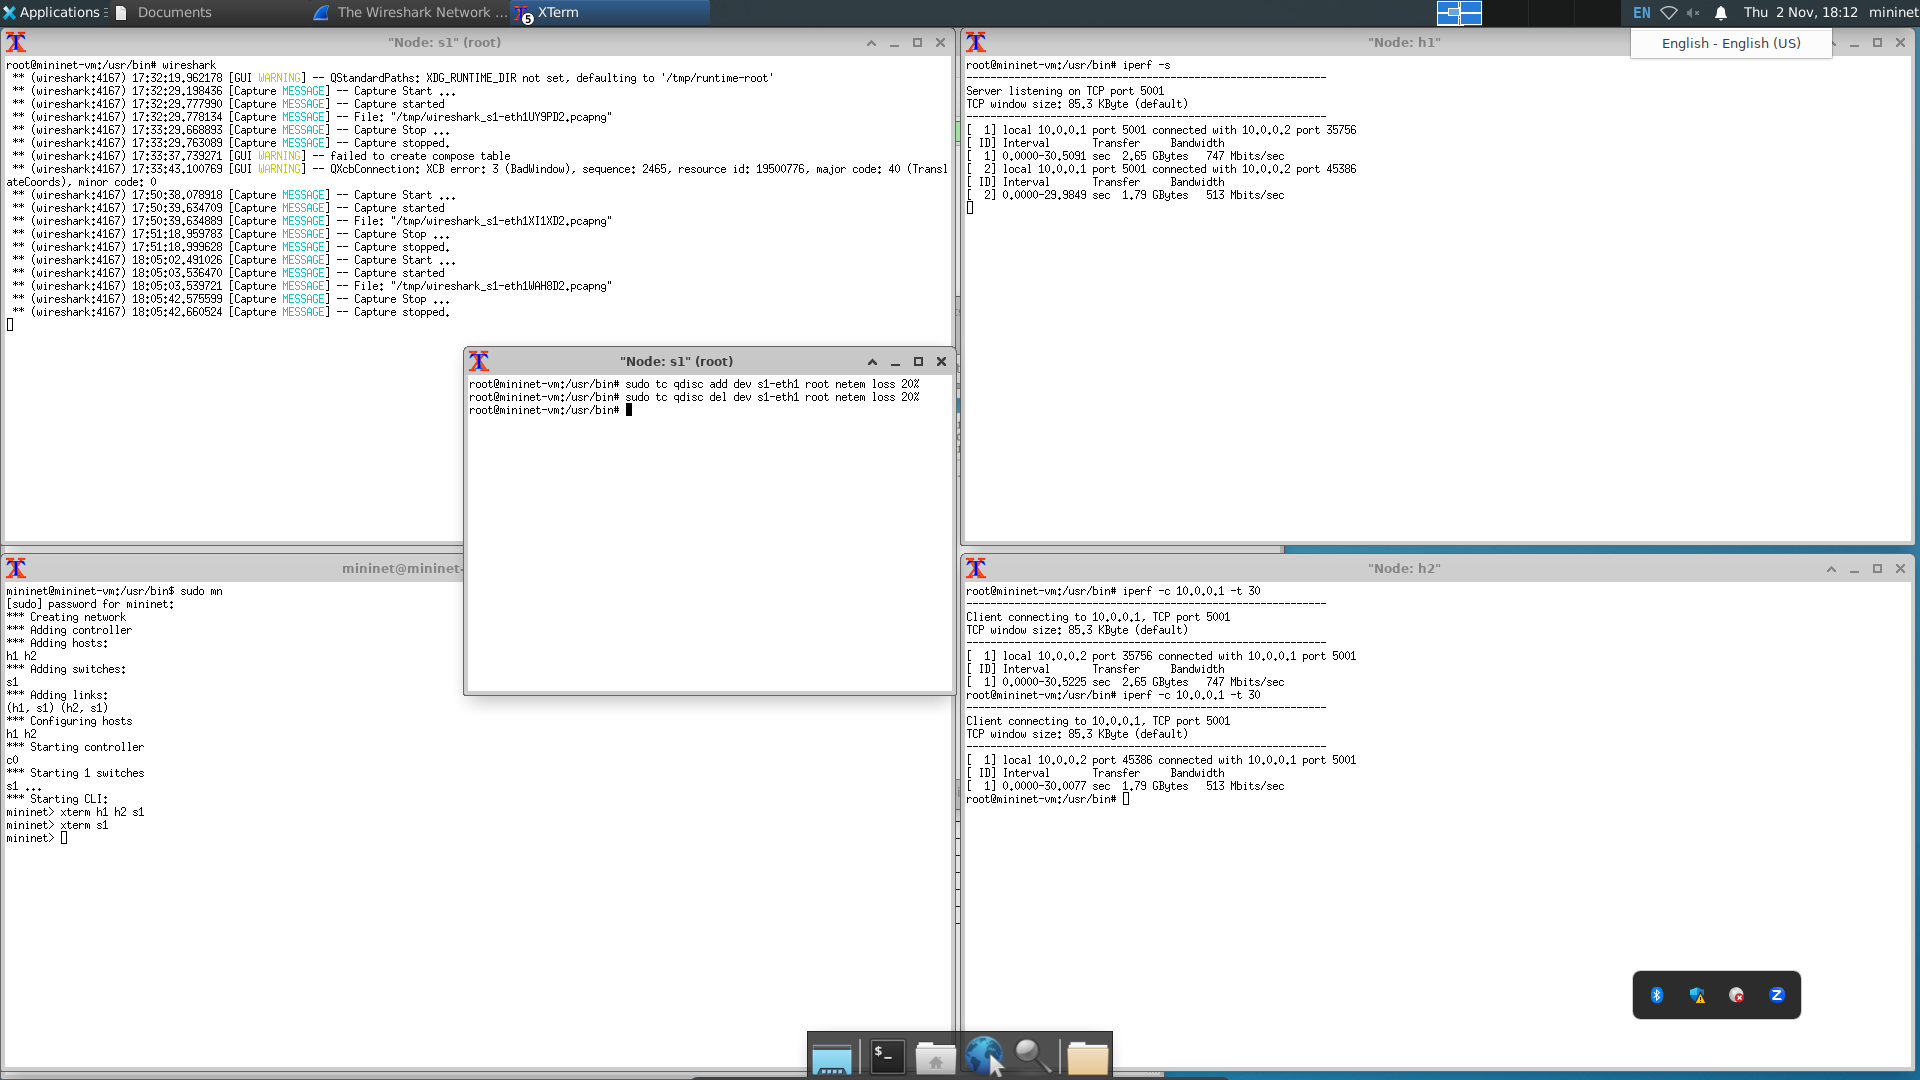
\includegraphics[width=11cm]{screenshot}
    \captionof{figure}{Terminals}

    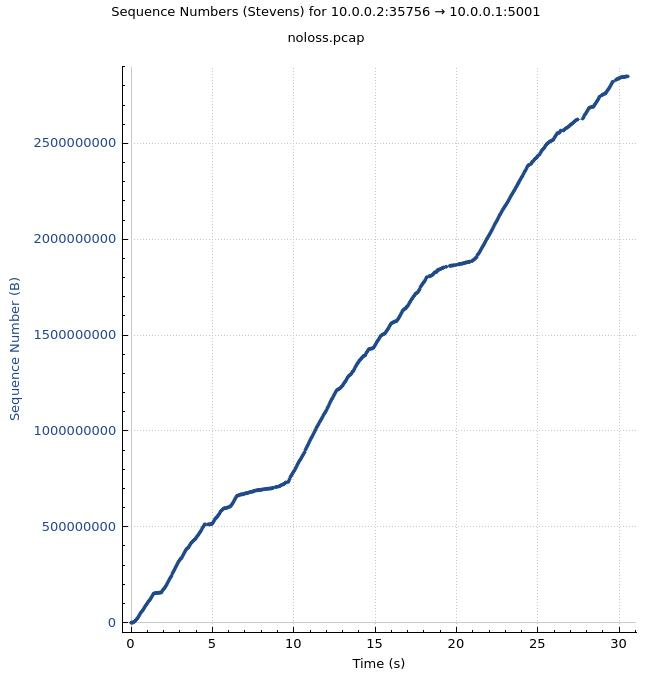
\includegraphics[width=8cm]{nolossstevens}
    \captionof{figure}{No Loss Stevens}
    
    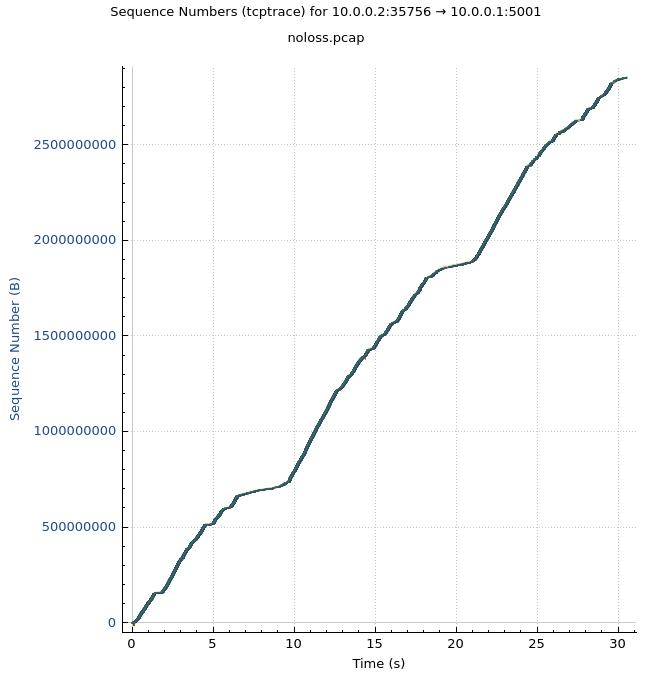
\includegraphics[width=8cm]{nolosstcptrace}
    \captionof{figure}{No Loss Tcptrace}

    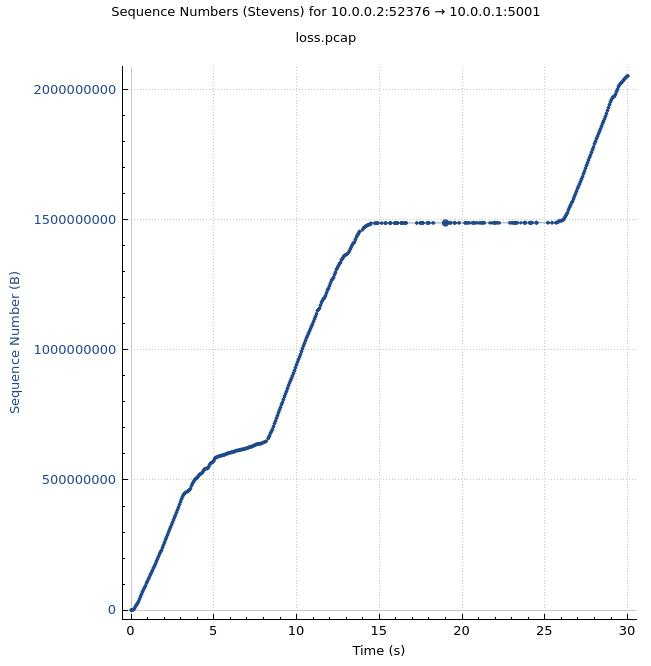
\includegraphics[width=8cm]{lossstevens}
    \captionof{figure}{Loss Stevens}
    
    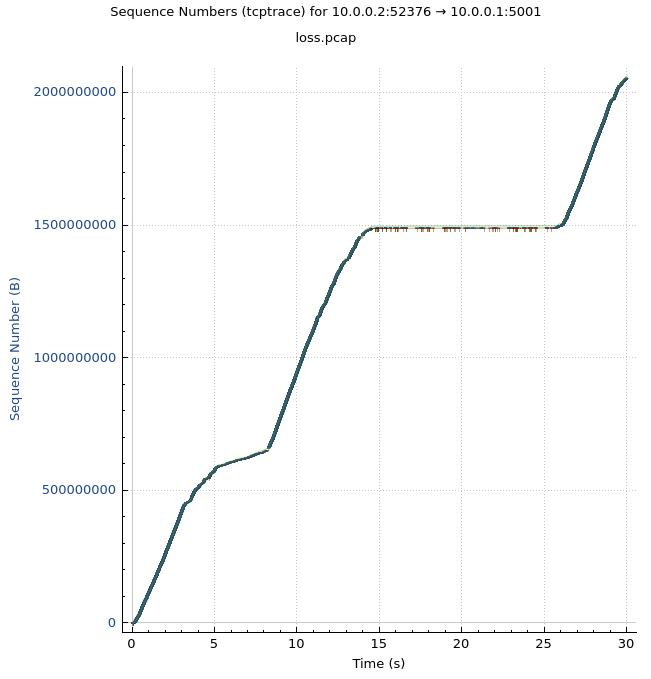
\includegraphics[width=8cm]{losstcptrace}
    \captionof{figure}{Loss Tcptrace}

    \section*{Questions}
    \subsection*{No Loss}
    On the time-sequence graph (tcp trace) with no loss, identify the regions of slow start
and congestion avoidance.

    \subsection*{Loss}
    On the time-sequence graph in the loss case, identify the region where the loss started
    Identify areas where slow start and congestion avoidance was used.
    Did you see any occurrence of fast recovery? If so, did it affect the congestion window?
    Is there a difference in throughput for the case with loss and no loss?
\end{document}